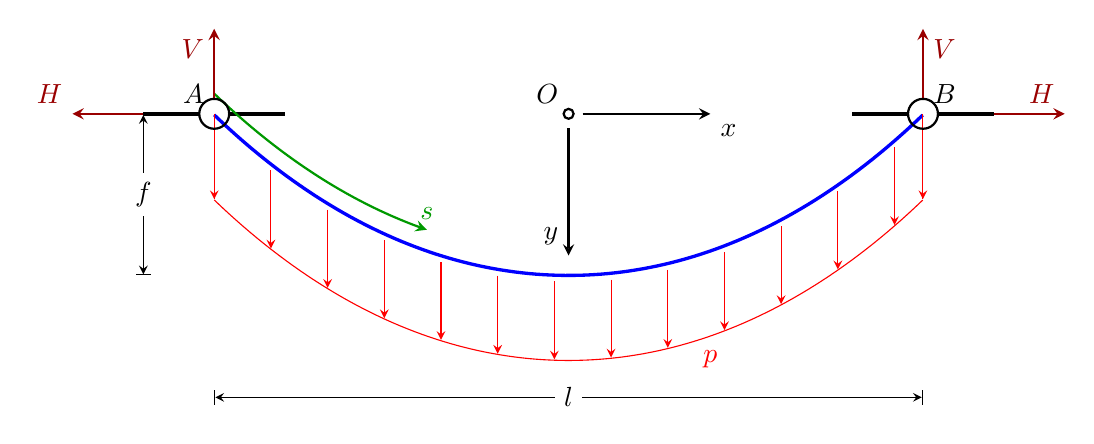
\begin{tikzpicture}[scale=1.8, >=stealth]
% Stile per i vincoli (muro/soffitto)
\tikzset{ground/.style={fill,pattern=north east lines,draw=none,minimum width=0.75cm,minimum height=0.3cm}}

% Parametri geometrici della catenaria per il plot matematico
\def\l{5}       % Luce (lunghezza totale)
\def\f{1.14}    % Freccia
\def\a{2.93}    % Parametro della catenaria per avere f=1.14 con l=5
\def\yv{1.86}   % Quota del vertice in mezzeria (3 - 1.14)

% Coordinate dei supporti
\coordinate (A) at (0,3);
\coordinate (B) at (5,3);
\coordinate (HA) at (-0.5,3);
\coordinate (HB) at (5.5,3);
\coordinate (VA) at (0,3.1);
\coordinate (VB) at (5,3.1);
\coordinate (O) at (2.5, 3);

% Rappresentazione dei supporti fisici
\draw[ultra thick] (-0.5,3) -- (-0.1,3);
\draw[ultra thick] ( 0.1,3) -- (0.5,3);
\draw[ultra thick] (4.5,3)  -- (4.9,3);
\draw[ultra thick] (5.1,3)  -- (5.5,3);

% --- LA FUNE (CATENARIA REALE) ---
% Equazione: y = yv + a * (cosh((x-2.5)/a) - 1) espressa in forma esponenziale
\draw[very thick, blue, samples=100, domain=0:\l] 
    plot (\x, {\yv + \a*(0.5*(exp((\x-2.5)/\a) + exp(-(\x-2.5)/\a)) - 1)});

% --- TRATTO DI ASCISSA CURVILINEA s (PARALLELA ALLA CATENARIA) ---
\draw[->, green!60!black, thick, samples=50, domain=0:1.5] 
    plot (\x, {\yv + \a*(0.5*(exp((\x-2.5)/\a) + exp(-(\x-2.5)/\a)) - 1) + 0.15});

% Posizionamento della lettera 's' sopra la punta della freccia verde
\pgfmathsetmacro{\xS}{1.5}
\pgfmathsetmacro{\yS}{\yv + \a*(0.5*(exp((\xS-2.5)/\a) + exp(-(\xS-2.5)/\a)) - 1) + 0.15}
\node[green!60!black, above] at (\xS,\yS) {$s$};

% --- CARICO DISTRIBUITO LUNGO LA FUNE (PESO PROPRIO) ---
% Profilo superiore del carico (offset di +0.6 verticalmente rispetto alla catenaria)
\draw[red, thin] plot[samples=100, domain=0:\l] 
    (\x, {\yv + \a*(0.5*(exp((\x-2.5)/\a) + exp(-(\x-2.5)/\a)) - 1) - 0.6});

% Chiusure laterali del diagramma di carico agli appoggi
\draw[red, thin] (0,3) -- (0,2.4);
\draw[red, thin] (5,3) -- (5,2.4);

% Generazione delle frecce di carico verticali che seguono l'andamento della fune
\foreach \x in {0, 0.4, 0.8, 1.2, 1.6, 2.0, 2.4, 2.8, 3.2, 3.6, 4.0, 4.4, 4.8, 5.0} {
    \pgfmathsetmacro{\yline}{\yv + \a*(0.5*(exp((\x-2.5)/\a) + exp(-(\x-2.5)/\a)) - 1.22)}
    \draw[->, red, thin] (\x, {\yline + 0.6}) -- (\x, {\yline + 0.05});
}
% Etichetta del carico costante lungo la curva
\node[red, below] at (3.5, 1.4) {$p$};

% --- QUOTE ---
\draw[black, thin, |<->|] (0, 1) -- (5, 1) node[midway, fill=white] {$l$};
\draw[black, thin, |<->|] (-0.5, 3) -- (-0.5, 1.86) node[midway, fill=white] {$f$};

% --- SISTEMA DI RIFERIMENTO ---
\draw[thick] (O) circle (1pt) node[above left] {$O$};
\draw[->, black, thick] (2.6, 3 ) -- (3.5, 3) node[below right]{${x}$};
\draw[->, black, thick] (2.5, 2.9 ) -- (2.5, 2) node[above left]{${y}$};

% Tensioni agli estremi
\draw[->, red!60!black, thick] (VA) -- ++( 0.0, 0.5) node[below left] {${V}$};
\draw[->, red!60!black, thick] (VB) -- ++( 0.0, 0.5) node[below right] {${V}$};
\draw[->, red!60!black, thick] (HA) -- ++(-0.5, 0.0) node[above left] {${H}$};
\draw[->, red!60!black, thick] (HB) -- ++( 0.5, 0.0) node[above left] {${H}$};

% Nodi di testo per i punti
\draw[thick] (A) circle (3pt) node[above left] {$A$};
\draw[thick] (B) circle (3pt) node[above right] {$B$};

\end{tikzpicture}